\chapter{Software Testing}
\label{chap:softwareTesting}

The very famous quote of Paul, ``To err is human, but to really foul things up you need a computer, is quite relevant to the software programmers. Programmers being humans are prone to errors. Therefore, in spite of the best efforts, some errors may remain in the software after its completion.  Errors cannot be tolerated in software because a single error may cause a large upset in the system. According to the National Institute of Standard and Technology \cite{Tassey2002}, software errors cost an estimated \$59.5 billion loss to US economy annually. The destruction of Mariner 1 rocket (1962) costing \$18.5 million was due to a small error in formula coded incorrectly by programmer. The Hartford Coliseum Collapse (1978) costing \$70 million, Wall Street crash (1987) costing \$500 billion, failing of long division by Pentium (1993) costing \$475 million, Ariane 5 Rocket disaster costing \$500 million and many others were caused by minor errors in the software \cite{toweysoftware}. To achieve high quality, the software has to satisfy rigorous stages of testing. The more complex the software, the higher the requirements for software testing and the larger the damage caused when a bug remains in the software.

\section{Software Testing}
In the IEEE standard glossary of software engineering terminology~\cite{american1984}, testing is defined as ``the process of exercising or evaluating a system or system component by manual or automated means to verify that it satisfies specified requirements and actual results. A successful test is one that finds a fault~\cite{Myers1979}, where fault denotes the error made by programmers during software development~\cite{american1984}.

The testing process, being an integral part of Software Development Life Cycle (SDLC), is started from requirement phase and continues throughout the life of the software. In traditional testing when tester finds a fault in the given SUT, the software is returned to the developers for rectification and is consequently given back to the tester for retesting. It is important to note that, ``program testing can be used to show the presence of bugs, but never to show the absence of bugs~\cite{Dijkstra1972}. In other words, a SUT that passes all the tests without giving a single error is not guaranteed to contain no error. However, the testing process increases reliability and confidence of users in the tested product.

\begin{table}[ht]
%\scriptsize
\caption{Parts of Software Testing~\cite{adrion1982validation, chilenski1994applicability, gaudel2010software, richardson1992specification, tracey1998automated}} % title of Table
\smallskip
\centering % used for centering table
\begin{tabular}{| l | l | l | l | } % centered columns (4 columns)
\hline

Levels 					&Purpose		 				& Perspective			& Execution 	\\
\hline
1. Unit					&1. Functionality		& 1. White Box		& 1. Static 	\\
2. Integration	&2. Structural			& 2. Black Box		& 2. Dynamic	\\
3. System				&3. Robustness			& 								&			\\
								&4. Stress					&									&			\\
								&5. Compatibility		&									&			\\
								&6. Performance			&									&			\\



\hline %inserts single line
\end{tabular}
\bigskip
\label{table:addvalues} % is used to refer this table in the text
\end{table}


\subsection{Software Testing Levels}
The three main levels of software testing defined in the literature include unit testing, integration testing and system testing~\cite{chilenski1994applicability}. Unit testing involves evaluation of piece-by-piece code and each piece is considered as independent unit. Units are combined together to form components. Integration testing ensures that the integration of units in a component is working properly. System testing is called out to make sure that the system formed by combination of components performs correctly to give the desired output.

\subsection{Software Testing Purpose}
The primary purpose of software testing is identification of faults in the given SUT for necessary correction in order to achieve high quality. Maximum number of faults can be identified if software is tested exhaustively. In exhausting testing SUT is checked against all possible combinations of input data, and the results obtained are compared with the expected results for assessment. Exhaustive testing is not always possible in most scenarios because of limited resources and infinite number of input values that software can take. Therefore, the purpose of testing is generally directed to achieve confidence in the system involved from a specific point of view. For example, functionality testing is performed to check functional aspect for working correctly. Structural testing analyses the code structure for generating test cases in order to evaluate paths of execution and identification of unreachable or dead code. In robustness testing the software behaviour is observed in the case when software receives input outside the expected input range. Stress and performance testing aims at testing the response of software under high load and its ability to process different nature of tasks~\cite{cohen2005robustness}. Finally, compatibility testing is performed to see the interaction of software with underlying operating system.
 %As proper planning is the key to success for many projects this is often also true with software testing. A software test plan is a well defined document that defines the goal, scope, method, resources and time schedule of the testing.
%A software testing technique in which a software is tested with all possible combination of inputs. This technique can prove conclusively that the software meet its specification however exhaustive testing is seldom feasible because of the large input domain or too many paths in a software code. 

\subsection{Software Testing Perspective}
Testing activities can be split up into white-box and black-box testing on the basis of perspective taken. 

\subsubsection{White-box testing}
In white-box or structural testing, the testers must do need to know about the complete structure of the software and can do necessary modification, if so required. Test cases are derived from the code structure and test passes only if the results are correct and the expected code is followed during test execution~\cite{ostrand2002white}. Some of the most common White-box testing techniques are briefly defined:

\paragraph{Data Flow Analysis}
Data Flow Analysis is a testing technique that focuses on the input values by observing the behaviour of respective variables during the execution of the SUT~\cite{clarke1989formal}. In this technique a control flow graph (CFG), graphical representation of all possible states of program, of a SUT is drawn to determine the paths that might be traversed by a program during its execution. Test cases are generated and executed to verify its conformance with CFG on the basis of data. 

Normally, program execution implies input of data, operations on it according to the defined algorithm, and output of results. This process can be viewed as a flow of data from input to output in which data may transform into several intermediate results before reaching its final state. In the process several errors can occur e.g. references may be made to variables that don’t exist, values may be assigned to undeclared variables or the value of variables may be changed in an unexpected and undesired manner. It is the ordered use of data implicit in this process that is the central object of the technique to ensure that none of the aforementioned errors occur~\cite{fosdick1976data}.

\paragraph{Control flow analysis}
Control flow Analysis is a testing technique which takes into consideration the control structure of a given SUT. Control structure is the order in which the individual statements, instructions or function calls are executed. In this technique a control flow graph (CFG), similar to the one required in data flow analysis, is drawn to determine the paths that might be traversed by a program during its execution. Test cases are generated and executed to verify its conformance with CFG on the basis of control. For example to follow a specific path (also known as branch) between two or more choices at specific state. Efforts are made to ensure that the set of selected test cases execute all the possible control choices at least once. The effectiveness of the testing technique depends on controls measurement. Two of the most common measurement criteria defined by Vilkomir et al. are Decision/Branch coverage and Condition coverage \cite{vilkomir2003tolerance}. 

\paragraph{Code-based fault injection testing}
A technique in which additional code is added to the code of the SUT at one or more locations to analyse its behaviour in response to the anomaly \cite{voas1997software}. The process of code addition is called instrumentation which is usually performed before compilation and execution of software. The added code can be use for multiple reasons i.e. injection of fault to find the error handling behaviour of software, to determine the effectiveness of test procedure to check whether it discover the injected faults or to measure the code coverage achieved by the testing process.    

\subsubsection{Black-box testing}
In black-box or functional testing, the testers do not need to know about internal code structure of the SUT. Test cases are derived from the specifications and test passes if the result is according to expected output. Internal code structure of the SUT is not taken into any consideration~\cite{beizer1995black}. Some of the most common black-box testing techniques are briefly defined:

\paragraph{Use-case based testing}
A verification and validation technique that utilizes use-cases of the system to generate test cases. Use-case define functional requirements at a particular situation or condition of the system from actor's (user or external system) perspective. It consists of a sequence of actions to represent a particular behaviour of the system. A use case format include a brief description of the event, flow of events, preconditions, postconditions, extension points, context diagram and activity diagram. 
All the details required for test case is included in the use case, therefore, use case can be easily transformed into test case. 

% steps taken from presentation of Raional User Conference 2003. Check it for viva.

The main benefits of use case testing is cheap generation of test cases, avoidance of test duplication, improved test coverage, easier regression testing and early identification of missing requirements.  

\paragraph{Partition testing}
A testing technique in which the input domain of a given SUT is divided into sub-domain according to some rule and then tests are conducted in each sub-domain. The division in to sub-domain can be according to the requirements or specifications, structure of the code or according to the process by which the software was developed \cite{hamlet1990}. 

While the performance of partition testing is directly dependant on the quality of sub-domain \cite{weyuker1991analyzing}, it is often however difficult to divide the domain into equal partitions. Therefore, another version of partition testing called Proportional sampling strategy: guidelines for software testing practitioners \cite{Chan1996} is devised, in which the number of test cases selected from each partition is directly proportional to the size of the partition. Experiments performed by Ntafos \cite{ntafos1998random} confirm the better performance of proportional partition testing over partition testing.


\paragraph{Boundary value analysis}
Boundary Value Analysis (BVA) is a testing technique which is based on the rationale that errors tends to occur near the extremities of the input variables. Therefore in BVA the data set consists of values which are selected from the borders. According to IEEE standards \cite{radatz1990ieee}, boundary value is a value that corresponds to minimum or maximum input, internal or external value specified for a component or system. 

The BVA technique is also used in conjunction with partition testing where test values are selected at the borders of each sub-domain instead of the whole input domain. The empirical analysis performed by Reid et al. \cite{reid1997empirical} argue that BVA performs better in finding faults than partition testing. They also stated that like partition testing the performance of BVA is also dependant on the correct identification of partition and selection of boundary values.

\paragraph{Formal specification testing}
Formal specification is defined as ``a mathematical based technique, which offers rigorous and effective way to model, design and analyse computer systems" \cite{formal1997specification, Hierons2009}. The mathematical structure allows formal specifications to be manipulated mechanically so that information contained within the specification can be isolated, transformed, assembled, and repackaged to be used as test cases. Furthermore, it also guarantee that the test frames are logical consequences of the specification \cite{donat1997automating}. Formal specification testing is effective because it is independent from the code of the SUT. Which means that no change is required in the test cases as long as the specifications are unchanged \cite{gaudel2010software}. It uses the existing specification model to verify the test results and thus avoid the oracle problem \cite{bertolino2007software}.


%\section{Common Techniques of Software Testing}
%This section briefly define some of the most common techniques of software testing currently being used in the testing industry. These include techniques from both white-box and black-box testing techniques.

% Check wikipedia for them.


%\subsubsection{Grey-Box Testing}
%Grey-Box testing is the combination of both black-box/functionality and white-box/structural testing. The tester knows about both the functionality and the internal structure of the SUT. Some of the test cases are based on the functionality and some of the test cases are based on the structure. Emphasis of grey-box testing is both on code coverage as well as functionality~\cite{Savenkov2008}.

%\subsection{Software Testing Workflow}
%There are many software techniques like unit testing, integration testing, random testing, regression testing, system testing, acceptance testing, performance testing, load testing, stress testing, alpha testing, beta test etc. All testing techniques belong to black-box, white-box or grey-box approach. Each testing technique has its own strength and weaknesses but the technique in focus here is Random Testing.


%\begin{figure}[h]
%\begin{center}
%	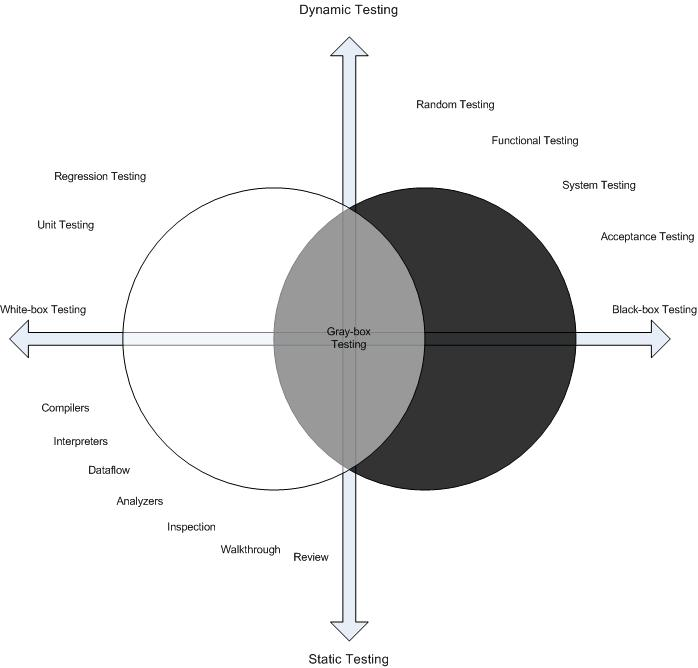
\includegraphics[width=16cm, height=12cm ]{Literature/Drawing34.jpg}
%	\caption{Software Testing Workflow}
%\end{center}  
%\end{figure}


%We have explained software testing graphically with the help of plotting venn diagram on two dimensional axis. The positive x axis represent black-box while negative x axis represent white-box testing. Grey-box testing in the middle is represented by the overlapping of black-box and white-box testing. Similarly on positive y axis we have dynamic testing and on negative y axis we have static testing.
%Now if a test is black box and dynamic then the test will fall in 0 to 90 degree on the diagram and if the test is black-box and static then it will fall in 270 to 360 degree. On the other hand if the test is white-box and dynamic then it will fall in 90 to 180 degree and if the test is white-box and static then it will fall in 180 to 270 degrees.




\subsection{Software Testing Execution}
Testing process can be divided into static and dynamic phases on the basis of test execution. In static testing test cases are analysed statically for checking errors without test execution. In addition to software code, high quality softwares are accompanied by necessary documentation. It includes requirements, design, technical, user manual marketing information. Reviews, walkthroughs or inspections are most commonly used techniques for static testing. In dynamic testing the software code is executed and input is converted into output. Results are analysed against expected outputs to find any error in the software. Unit testing, integration testing, system testing, and acceptance testing are most commonly used as dynamic testing methods~\cite{fairley1978tutorial}.

%Dynamic testing can be manual or automated. In manual testing the programmer develops the test cases which are executed by the developed software to find any error in processing or output. Similarly in automated testing the software or components of the software is given as input to testing software that automatically generates test cases and executes the SUT against them to find any errors. Manual testing typically consumes more time and resources than automated testing.



\subsubsection{Manual Testing}
Manual testing is the technique of finding faults in software in which the tester writes the code by hand to create test cases and test oracle~\cite{Ciupa2008}. Manual testing may be effective in some cases but it is generally laborious, time consuming and error-prone~\cite{tretmans1999}. Additionally, it requires that the testers must have appropriate skills, experience and sufficient knowledge of the SUT for evaluation from different perspectives.
 
\subsubsection{Automated Testing}
Automated testing is the technique of finding faults in a software in which the test cases or test oracle are generated automatically by a testing tool~\cite{Leitner2007}. There are tools which can automate part of a test process like generation of test cases or execution of test cases or evaluation of results while other tools are available which can automate the whole testing process. The use of automated testing made it possible to test large volumes of code, which would have been impossible otherwise~\cite{ramamoorthy1975testing}.

%\section{Automated Random Testing}
%\subsection{Test Data Generation}
%\subsection{Test Execution}

\subsubsection{Test Oracle}
Test oracles set the acceptable behaviour for test executions~\cite{baresi2001test}. All software-testing techniques depend on the availability of test oracle~\cite{gaudel2010software}. Designing test oracle for ordinary software may be simple and straightforward. However, for relatively complex software designing of oracle is quite cumbersome and requires special ways to overcome the oracle problem. Some of the common issues in the oracle problem include:
\begin{enumerate}
\item The assumption that the test results are observable and can be compared with the oracle.
\item An ideal test oracle would satisfy desirable properties of program specifications~\cite{baresi2001test}.
\item A specific oracle to satisfy all conditions is seldom available as rightly pointed out by Weyuker, stating that truly general test oracles are often unobtainable~\cite{weyuker1982testing}. 
\end{enumerate}

%\subsection{Test Report}

\subsection{Summary}

\section{Conclusion}


% ------------------------------------------------------------------------


%%% Local Variables:
%%% mode: latex
%%% TeX-master: "../thesis"
%%% End:
